\documentclass{article}
\usepackage[utf8]{inputenc}
\usepackage{amsmath, amsthm, amssymb, amsfonts}
\usepackage{tikz}
\usepackage{graphicx}
\graphicspath{ {./images/} }


\title{Homework 6}
\author{DUMA Yehor (31209504)}
\date{12/2}
\begin{document}

\maketitle

\section{Exercise 5}

$A = \{1,2,3,5,6,10,15,30\}$ \\
$R$ = $\{<x,y>|\hspace{2mm} x$ divides $y$ without remainder\} \\ \\
$R = \{ \langle 1,1 \rangle, \langle 2,2 \rangle,\langle 3,3 \rangle,\langle 5,5 \rangle,\langle 10,10 \rangle, \langle 15,15 \rangle, \langle 30,30 \rangle, \langle 1,2 \rangle, \langle 1,3 \rangle, \langle 1,5\rangle\, \langle 1,6 \rangle, \langle 1,10 \rangle, \\ \langle 1,15 \rangle, \langle 1,30 \rangle, \langle 2,6 \rangle, \langle 2,10 \rangle, \langle 2,30 \rangle, \langle 3,6 \rangle, \langle 3,15 \rangle, \langle 3,30 \rangle, \langle 5,10 \rangle, \langle 5,15 \rangle, \langle 5,30 \rangle, \langle 6,30 \rangle, \langle 10,30 \rangle, \langle 15,30 \rangle\}$ \\ \\
$R$ is \textbf{reflexive}, \textbf{anti-symmetric}, transitive,  \textbf{nonconnected}. \\ \\
Since $R$ is reflexive and anti-symmetric, it is a \textbf{weak order}. \\
Since $R$ is nonconnected, it is a \textbf{partial} (not total) order. \\ \\  \\
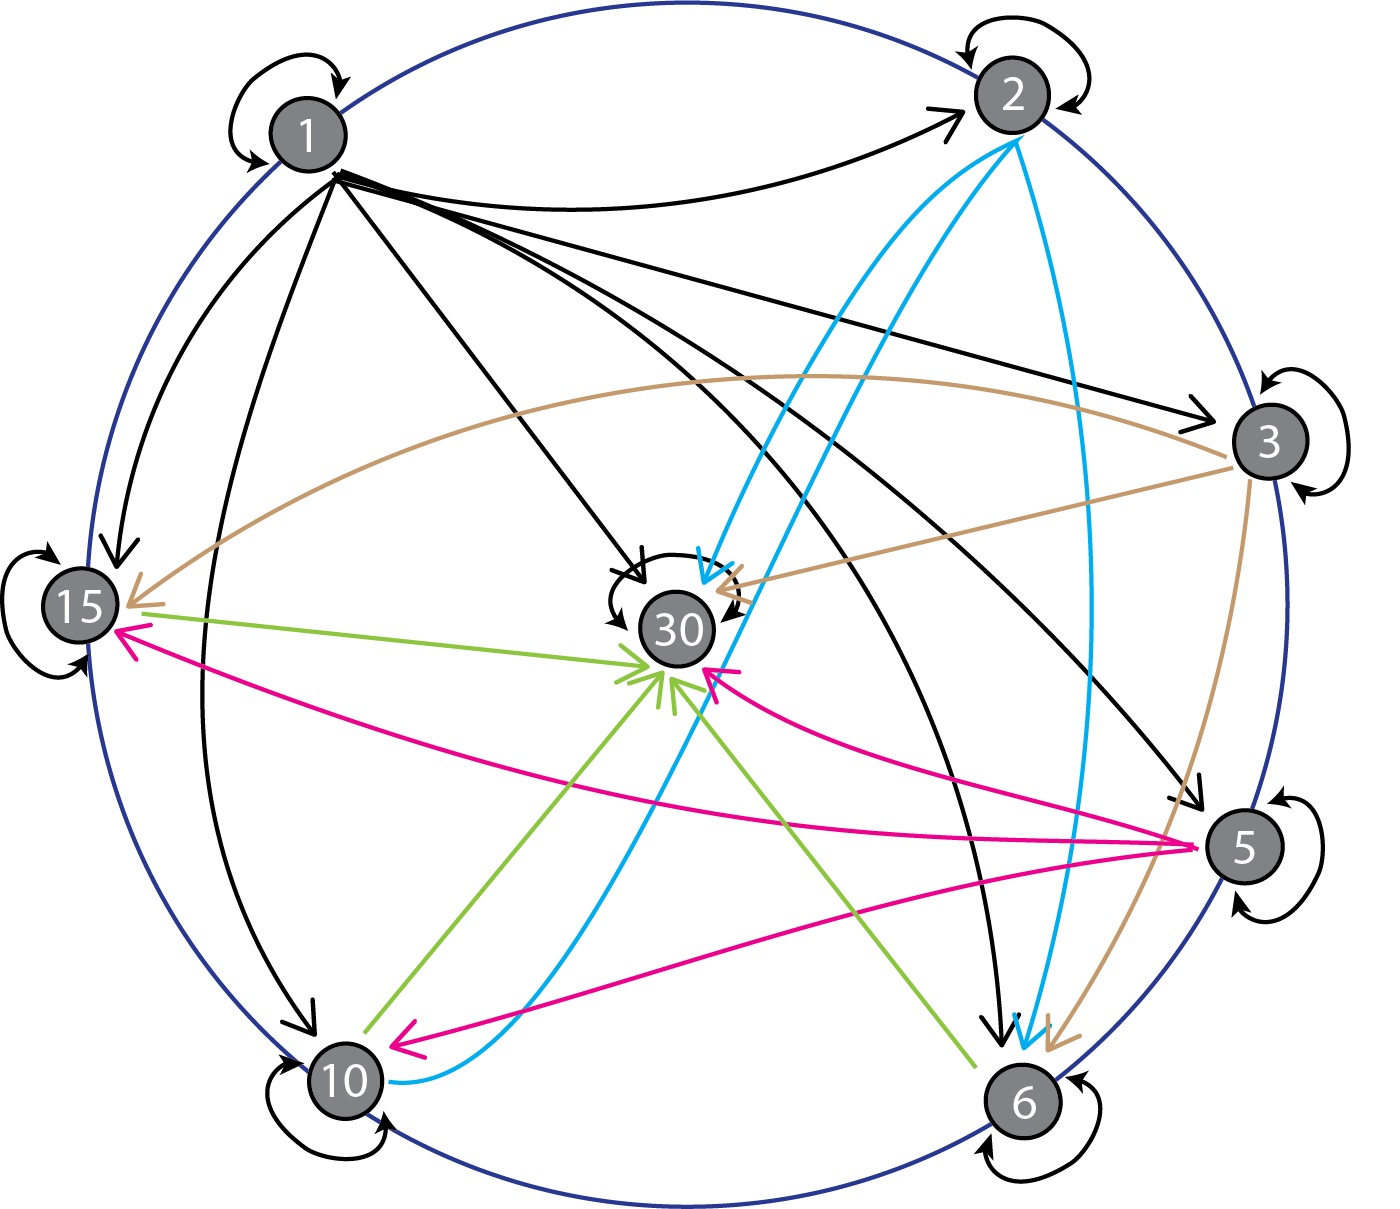
\includegraphics[scale=0.85]{nakazawa1} \\
\textbf{Minimal: 1 \\
Least: 1 \\
Maximal: 30 \\
Greatest: 30} \\ \\
$B = \{a,b,c\}$ \\
$\wp (B)=\{\{a\}, \{b\}, \{c\}, \{a,b\}, \{a,c\},\{b,c\},\{a,b,c\},\varnothing\} \\~\\$
$R$ = $\{<x,y>|\hspace{2mm}x$ is a subset of $y$\} \\ 
$R$ = \\ $\{\langle {\{a\}, \{a\} \rangle,\langle {\{b\}, \{b\} \rangle,\langle {\{c\}, \{c\} \rangle,\langle {\{a,b\}, \{a,b\} \rangle,\langle {\{a,c\}, \{a,c\} \rangle, $ \\ $\langle {\{b,c\}, \{b,c\} \rangle,\langle {\{a,b,c\}, \{a,b,c\} \rangle,\langle {\{a\}, \{a,b\} \rangle,\langle {\{a\}, \{a,c\} \rangle,\langle {\{a\}, \{a,b,c\} \rangle,$ \\ $\langle {\{b\}, \{a,b\} \rangle,\langle {\{b\}, \{b,c\} \rangle,\langle {\{b\}, \{a,b,c\} \rangle,\langle {\{c\}, \{a,c\} \rangle,\langle {\{c\}, \{b,c\} \rangle,$ \\ $\langle {\{c\}, \{a,b,c\} \rangle,\langle {\{a,b\}, \{a,b,c\} \rangle,\langle {\{b,c\}, \{a,b,c\} \rangle,\langle {\{a,c\}, \{a,b,c\} \rangle,$ \\ $\langle {\varnothing,\varnothing \rangle,\langle {\varnothing, \{a\} \rangle,\langle {\varnothing, \{b\} \rangle,\langle {\varnothing, \{c\} \rangle,\langle {\varnothing, \{a,b\} \rangle,\langle {\varnothing, \{a,c\} \rangle,\langle {\varnothing, \{b,c\} \rangle,\langle {\varnothing, \{a,b,c\} \rangle\}$
\\ \\
$R$ is \textbf{reflexive}, \textbf{anti-symmetric}, transitive,  \textbf{nonconnected}. \\
Since $R$ is reflexive and anti-symmetric, it is a \textbf{weak order}. \\
Since $R$ is nonconnected, it is a \textbf{partial} (not total) order. \\ \\
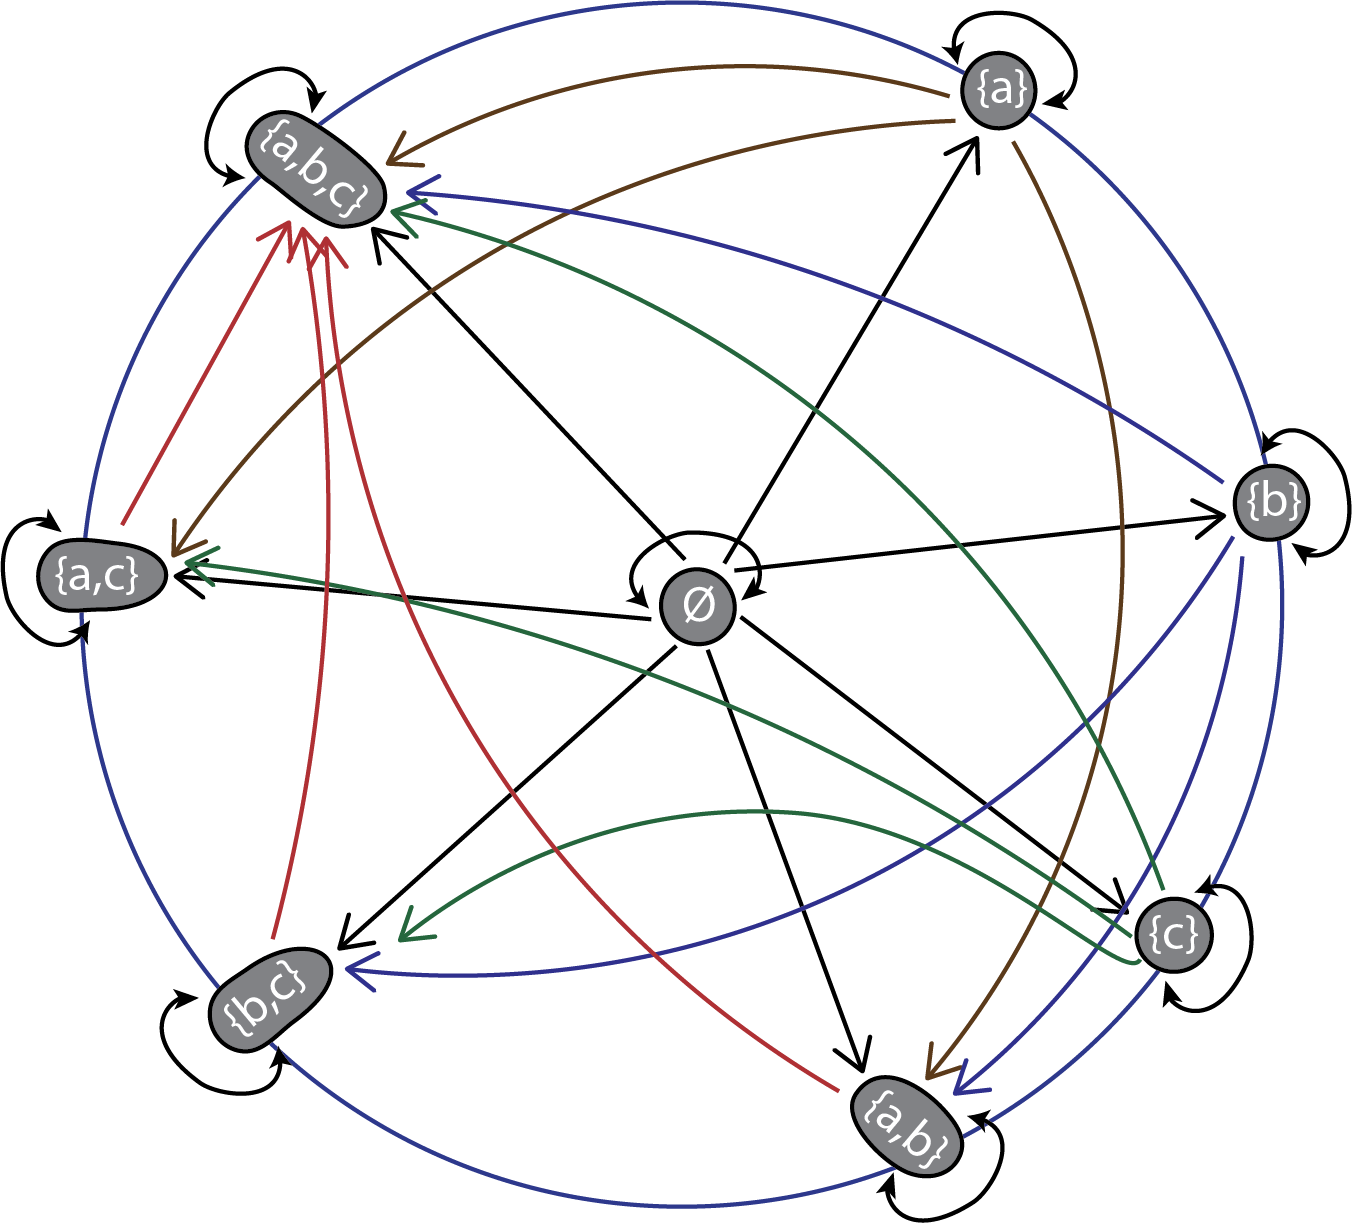
\includegraphics[scale=0.85]{nakazawa2} \\ \\ 
\textbf{Minimal: $\varnothing$} \\
\textbf{Least: $\varnothing$} \\
\textbf{Maximal: $\{a,b,c\}$} \\
\textbf{Greatest: $\{a,b,c\}$}
\end{document}